\documentclass{article}




\usepackage{fullpage}
%\usepackage{nopageno}
\usepackage{amsmath}
\usepackage{amsfonts}
\usepackage{graphicx}
\usepackage{framed}
\usepackage{algorithmic}
\usepackage{xcolor}

\definecolor{dark_red}{rgb}{0.5,0.0,0.0}
\definecolor{dark_green}{rgb}{0.0,0.5,0.0}
\definecolor{dark_blue}{rgb}{0.0,0.0,0.5}
\definecolor{blue}{rgb}{0.0,0.0,1.0}

\newcommand{\dr}[1]{\textcolor{dark_red}{#1}}
\newcommand{\dg}[1]{\textcolor{dark_green}{#1}}
\newcommand{\db}[1]{\textcolor{dark_blue}{#1}}
\newcommand{\blue}[1]{\textcolor{blue}{#1}}


\title{Using nested dissection to solve problems in electrostatics} 
\date{}

\begin{document}

\maketitle

\begin{abstract}
The ``nested dissection" of linear systems remains a powerful tool for solving linear systems that cover large computational meshes. The example application that will be addressed here will be the problem of computing the voltages at all points within a volume given the voltage at each point on the surface. The focus will be on solving the linear system as opposed to the setup of the linear system. The computational complexity of the nested dissection approach for a 3D computational mesh will be analyzed and compared with other approaches. Other benefits of nested dissection will also be addressed. 
\end{abstract}






\section{Finite element model for electrostatics} 

\begin{center}
\begin{tabular}{cc}
\parbox{0.5\textwidth}{
The problem that will be addressed here is the problem of computing the static voltage in the interior of a volume, given the voltages on the surface of said volume. The differential equation that is to be solved is Laplace's equation:
\[\nabla^2 V = 0\]
where \(V\) is voltage, and the boundary condition is that the value of \(V\) on the surface of the volume is known.

A large mesh is used to cover the volume, and the vector of voltages at each node in the interior of the mesh (\(\vec{V}_{\text{interior}}\)) is desired, while the voltages on the exterior of the mesh (\(\vec{V}_{\text{boundary}}\)) are given. The finite element method is used to create a linear system from which the net electric flux out of each interior node is a linear function of the voltages on each node. This results in the following linear system: 
\[C_{\text{interior}}\vec{V}_{\text{interior}} + C_{\text{boundary}}\vec{V}_{\text{boundary}} = \vec{0}\]
} & \parbox{0.5\textwidth}{
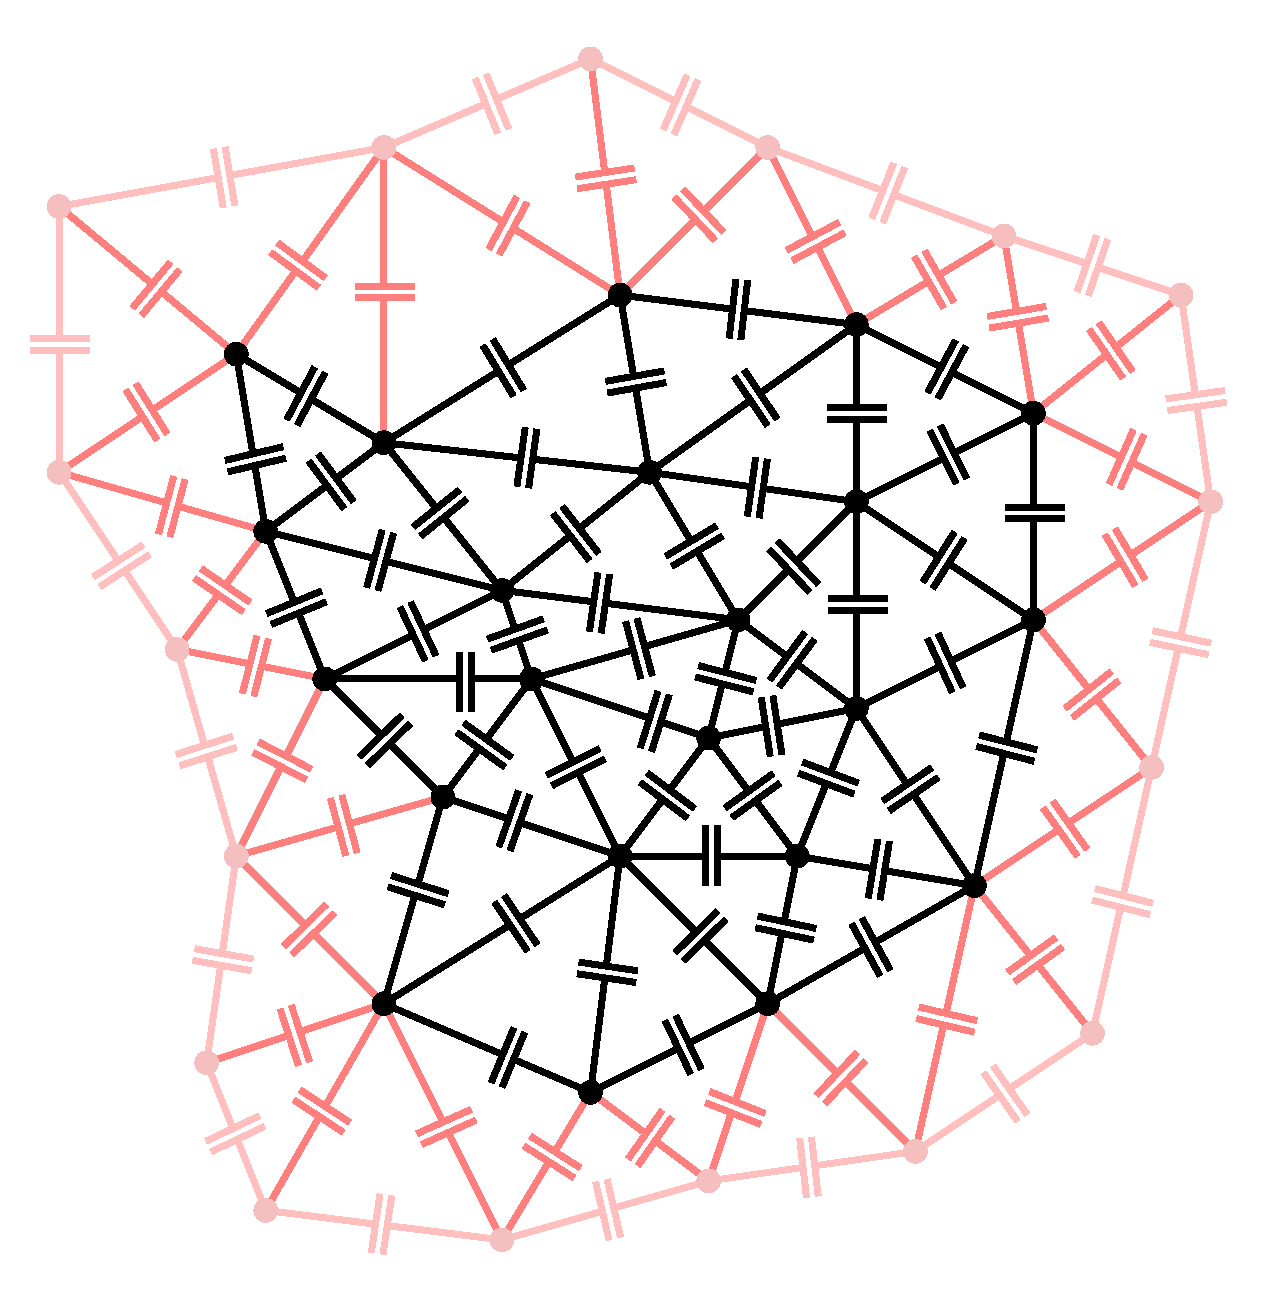
\includegraphics[width = 0.5\textwidth]{electrostatics_computational_mesh}
}
\end{tabular}
\end{center}

The aim is to find a solution matrix \(A\) such that knowing the voltages on the boundary \(\vec{V}_{\text{boundary}}\), the voltages on the interior \(\vec{V}_{\text{interior}}\) can be easily computed:

\[\vec{V}_{\text{interior}} = A\vec{V}_{\text{boundary}}\]

The solution matrix \(A\) will be derived by solving the system \(C_{\text{interior}}\vec{V}_{\text{interior}} + C_{\text{boundary}}\vec{V}_{\text{boundary}} = \vec{0}\) for the interior voltages \(\vec{V}_{\text{interior}}\), while leaving the boundary voltages \(\vec{V}_{\text{boundary}}\) as arbitrary values. This requires solving the system:
\[C_{\text{interior}}\vec{V}_{\text{interior}} = -C_{\text{boundary}}\vec{V}_{\text{boundary}}\]

The entries of both \(C_{\text{interior}}\) and \(C_{\text{boundary}}\) are measures of capacitance, and these matrices are symmetric. 

The dimensions of the 3D mesh will be assumed to have the same scale, in the sense that the mesh is not flat or linear. If \(O(N)\) is the scale of the width of the mesh in terms of the number of nodes, then 
\begin{itemize}
\item \(\vec{V}_{\text{interior}}\) has \(O(N^3)\) entries.
\item \(\vec{V}_{\text{boundary}}\) has \(O(N^2)\) entries. 
\item \(C_{\text{interior}}\) is an \(O(N^3) \times O(N^3)\) {\bf sparse} matrix.
\item \(C_{\text{boundary}}\) is an \(O(N^3) \times O(N^2)\) {\bf sparse} matrix.
\item The desired solution matrix \(A\) is an \(O(N^3) \times O(N^2)\) {\bf full} matrix.
\end{itemize} 

{\bf Without} exploiting the sparse structure of matrices \(C_{\text{interior}}\) or \(C_{\text{boundary}}\), solving the system requires \(O(N^9)\) flops. In the following sections, different approaches to exploiting the sparse structure of the matrices will be explored, including what is known as ``nested dissection".





\section{Sparse matrix approach}

A ``sparse" matrix \(M\) is represented by listing all of the non-zero elements. {\bf For the following discussion, the rows and columns of the matrix will be indexed not by numbers, but by variable names.} Each element has a row name, a column name, and the element's value. 

A sparse matrix is often represented through the use of a directed graph. Each node corresponds to a variable in the linear system: 
\[M\vec{x} = N\vec{y}\]
{\bf There are two types of variables: unknown variables, and conditioned variables.} 

Each unknown variable, which are the variables from \(\vec{x}\), has a linear equation (which may include a constant) associated with it, and this equation contains said variable as well as other variables from both \(\vec{x}\) and \(\vec{y}\). 

Each conditioned variable, which are the variables from \(\vec{y}\), is considered an arbitrary value. The values of the unknown variables are to be solved for in terms of the conditioned variables.

If variable \(x_j\) appears in the equation associated with \(x_i\), and the coefficient of \(x_j\) in said equation is \(a_{i,j}\), then the matrix entry with row indexed by \(x_i\) and column indexed by \(x_j\) has the value \(a_{i,j}\). This results in a directed edge with a weight of \(a_{i,j}\) starting at node \(x_j\) and terminating at node \(x_i\), as is depicted below. The diagonal entries, that is the entries whose row and column have the same name, will all be assumed to be nonzero otherwise some variables will not appear in their own equations. Constant terms have their own column in the sparse matrix.    

\begin{center} 
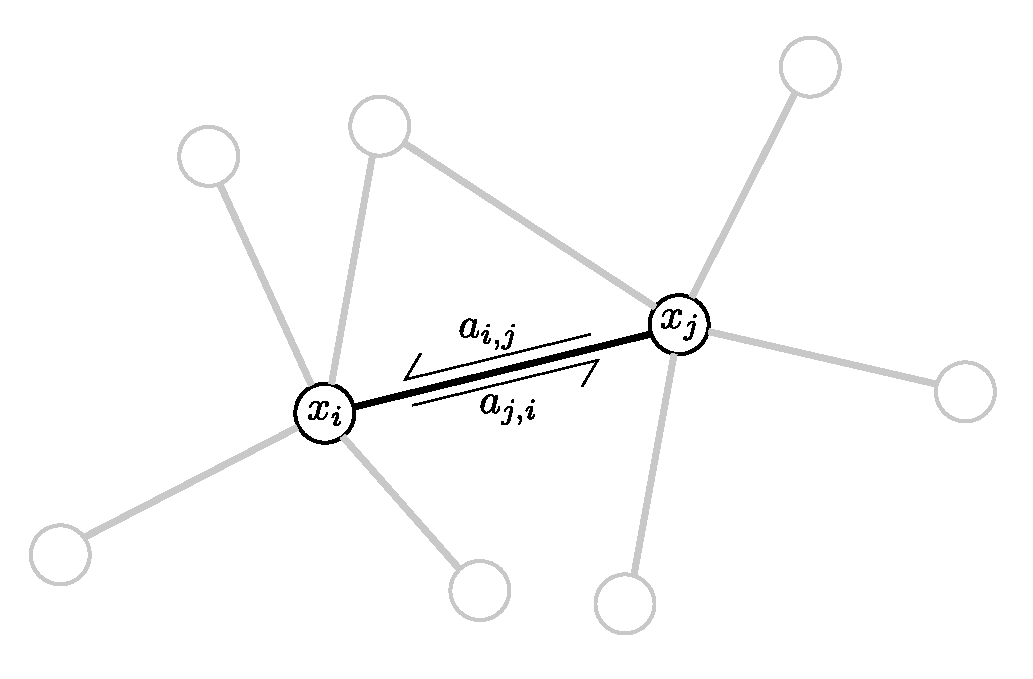
\includegraphics[width = 0.75\textwidth]{directed_graph_computational_mesh}
\end{center}

The aim is to solve for each of the unknown variables as linear functions of the conditioned variables. To achieve this, there are two stages: {\bf variable elimination} followed by {\bf back substitution}. 

With variable elimination, each of the unknown variables is in turn solved for using its own equation. The expression for said variable is then used to eliminate the variable in the equations corresponding to all other unknown variables except for variables that have already been eliminated. The variable is then considered ``eliminated". 

With back substitution, substitutions are made until all unknown variables are functions of the conditioned variable.   

When a variable, say \(X\), is eliminated, the equation for \(X\) is solved explicitly for \(X\) in terms of the other variables, the other variables being the variables with edges directed at \(X\). This expression for \(X\) will then be used to eliminate the appearance of \(X\) in the equations of other variables that depend on \(X\).   

In the image below, variables \(A_1\), \(A_2\), ..., \(A_a\), \(B_1\), \(B_2\), ..., \(B_b\) are the origin point of edges directed at \(X\). This means that the computed expression for \(X\) consists of \(A_1\), \(A_2\), ..., \(A_a\), \(B_1\), \(B_2\), ..., \(B_b\). 

Variables \(B_1\), \(B_2\), ..., \(B_b\), \(C_1\), \(C_2\), ..., \(C_c\), \(D_1\), \(D_2\), ..., \(D_d\) all depend on \(X\). Variables \(D_1\), \(D_2\), ..., \(D_d\) will be assumed to be variables that have already been eliminated, so their expressions will not be altered. 

During the elimination of variable \(X\), the expression for \(X\) in terms of \(A_1\), \(A_2\), ..., \(A_a\), \(B_1\), \(B_2\), ..., \(B_b\) will be used to replace \(X\) in the equations corresponding to the variables \(B_1\), \(B_2\), ..., \(B_b\), \(C_1\), \(C_2\), ..., \(C_c\). This means that for each of \(B_1\), \(B_2\), ..., \(B_b\), \(C_1\), \(C_2\), ..., \(C_c\), the inwards edge from \(X\) is instead replaced with inwards edges from \(A_1\), \(A_2\), ..., \(A_a\), \(B_1\), \(B_2\), ..., \(B_b\) (an edge to and from the same node is not added to the directed graph). The process has a computational complexity of \(O((a + b)(b + c))\) flops.

\begin{center} 
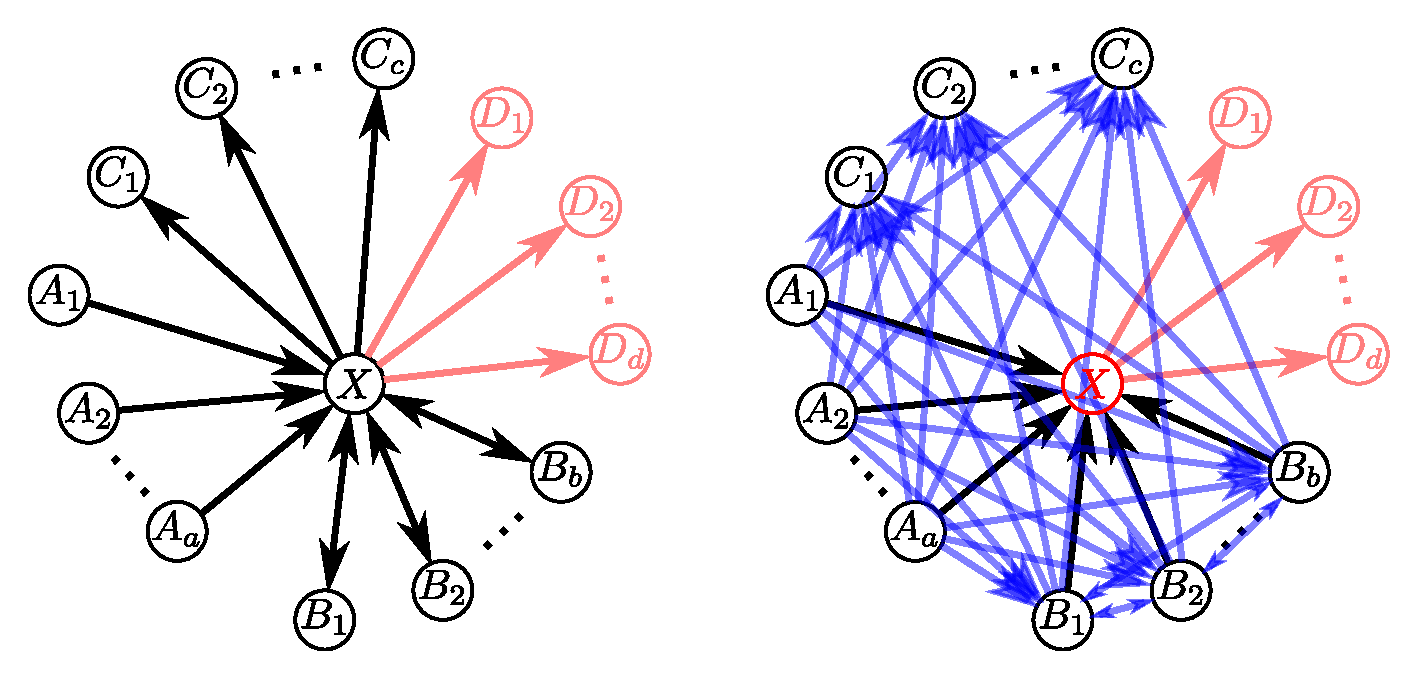
\includegraphics[width = 0.75\textwidth]{variable_mesh_elimination}
\end{center}

Nodes that correspond to conditioned variables are assigned arbitrary fixed values. They have no equation associated with them, nor do they have any inwards oriented edges. These nodes are not eliminated.

Below is depicted the process of the gradual elimination of nodes from a 2D computational mesh. Node are eliminated starting with the top left node, then following row by row. 

\begin{center}
\begin{tabular}{cccc}
\parbox{0.2\textwidth}{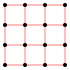
\includegraphics[width = 0.2\textwidth]{example_straight_forwards_elimination/example_straight_forwards_elimination_panel_1}} 
& \parbox{0.2\textwidth}{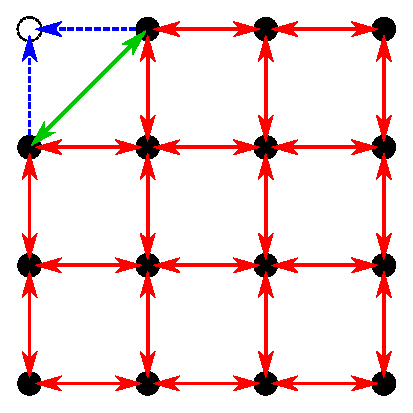
\includegraphics[width = 0.2\textwidth]{example_straight_forwards_elimination/example_straight_forwards_elimination_panel_2}} 
& \parbox{0.2\textwidth}{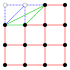
\includegraphics[width = 0.2\textwidth]{example_straight_forwards_elimination/example_straight_forwards_elimination_panel_3}} 
& \parbox{0.2\textwidth}{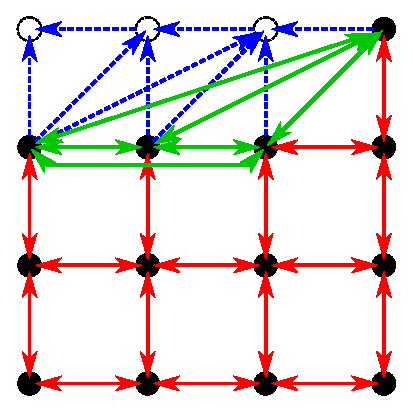
\includegraphics[width = 0.2\textwidth]{example_straight_forwards_elimination/example_straight_forwards_elimination_panel_4}} 
\\ \parbox{0.2\textwidth}{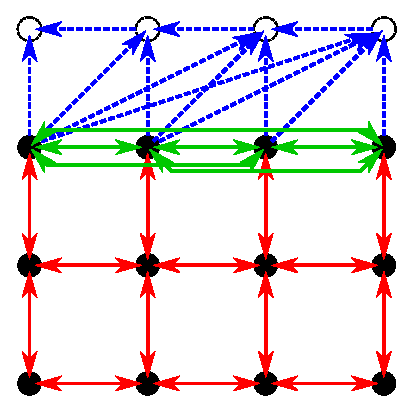
\includegraphics[width = 0.2\textwidth]{example_straight_forwards_elimination/example_straight_forwards_elimination_panel_5}} 
& \parbox{0.2\textwidth}{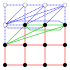
\includegraphics[width = 0.2\textwidth]{example_straight_forwards_elimination/example_straight_forwards_elimination_panel_6}} 
& \parbox{0.2\textwidth}{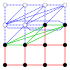
\includegraphics[width = 0.2\textwidth]{example_straight_forwards_elimination/example_straight_forwards_elimination_panel_7}} 
& \parbox{0.2\textwidth}{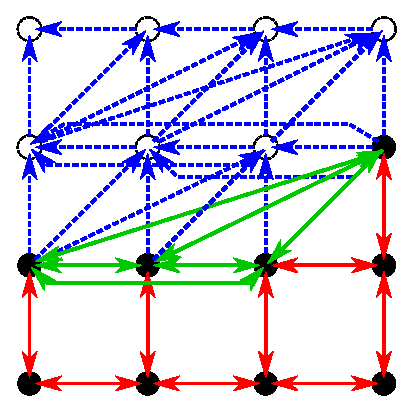
\includegraphics[width = 0.2\textwidth]{example_straight_forwards_elimination/example_straight_forwards_elimination_panel_8}} 
\\ \parbox{0.2\textwidth}{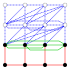
\includegraphics[width = 0.2\textwidth]{example_straight_forwards_elimination/example_straight_forwards_elimination_panel_9}} 
& \parbox{0.2\textwidth}{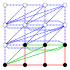
\includegraphics[width = 0.2\textwidth]{example_straight_forwards_elimination/example_straight_forwards_elimination_panel_10}} 
& \parbox{0.2\textwidth}{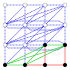
\includegraphics[width = 0.2\textwidth]{example_straight_forwards_elimination/example_straight_forwards_elimination_panel_11}} 
& \parbox{0.2\textwidth}{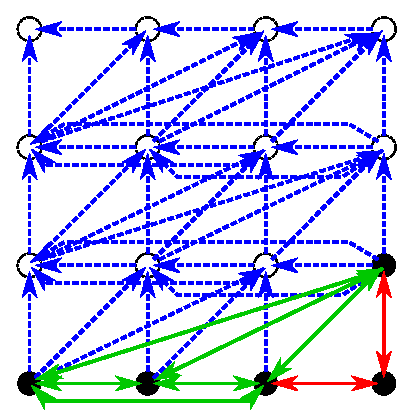
\includegraphics[width = 0.2\textwidth]{example_straight_forwards_elimination/example_straight_forwards_elimination_panel_12}} 
\\ \parbox{0.2\textwidth}{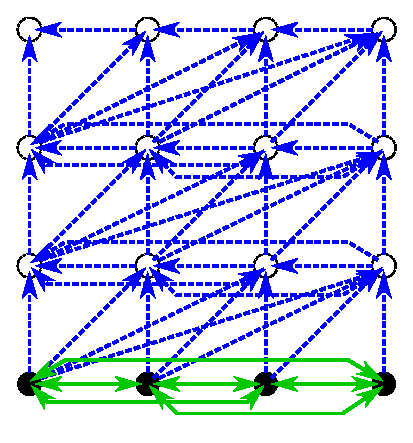
\includegraphics[width = 0.2\textwidth]{example_straight_forwards_elimination/example_straight_forwards_elimination_panel_13}} 
& \parbox{0.2\textwidth}{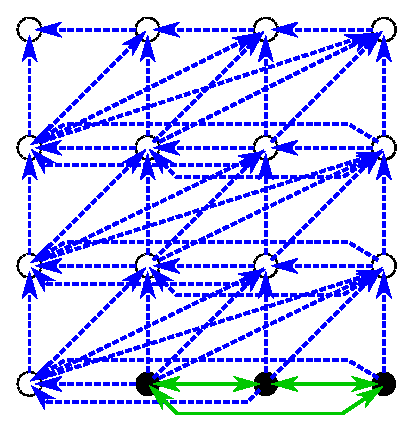
\includegraphics[width = 0.2\textwidth]{example_straight_forwards_elimination/example_straight_forwards_elimination_panel_14}} 
& \parbox{0.2\textwidth}{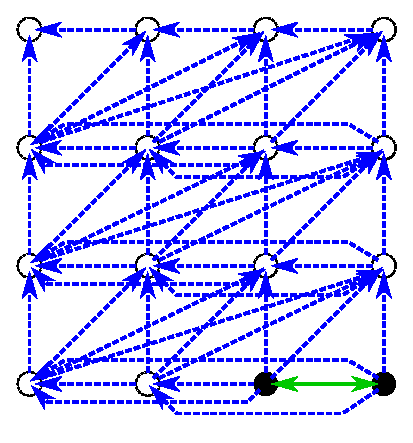
\includegraphics[width = 0.2\textwidth]{example_straight_forwards_elimination/example_straight_forwards_elimination_panel_15}} 
& \parbox{0.2\textwidth}{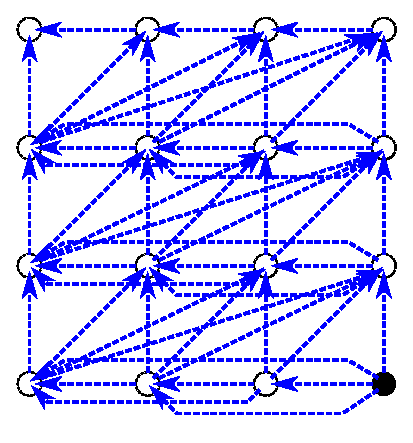
\includegraphics[width = 0.2\textwidth]{example_straight_forwards_elimination/example_straight_forwards_elimination_panel_16}} 
\end{tabular}
\end{center}

Once all unknown variables have been eliminated, the final step is ``back substitution". With back substitution, the expressions for variables that depend only on conditioned variables are recursively substituted into the expressions for other variables until all expressions depend only on the conditioned nodes. Back substitution is used to eliminate dependence on each unknown variable, typically processing each variable in the reverse order that they were eliminated in.  

In the image below, variables \(A_1\), \(A_2\), ..., \(A_a\), are the conditioned variables. The current expression for \(X\) consists of only \(A_1\), \(A_2\), ..., \(A_a\). 

Variables \(D_1\), \(D_2\), ..., \(D_d\) all depend on \(X\). During the process of back substitution, for each variable \(D_1\), \(D_2\), ..., \(D_d\), the appearance of \(X\) is replaced with the expression involving \(A_1\), \(A_2\), ..., \(A_a\), thereby eliminating \(X\) in the expressions associated with each of \(D_1\), \(D_2\), ..., \(D_d\). The process has a computational complexity of \(O(a \cdot d)\) flops. The computational complexity of back substitution is almost always cheaper than variable elimination.  

\begin{center} 
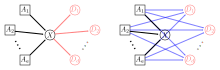
\includegraphics[width = 0.75\textwidth]{variable_mesh_back_substitution}
\end{center}

Below is depicted variable elimination where conditioned variables are present and depicted using squares. 

\begin{center}
\begin{tabular}{cccc}
\parbox{0.2\textwidth}{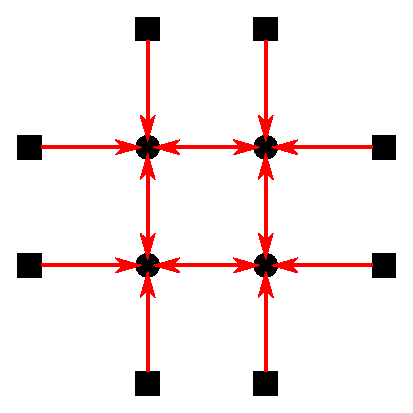
\includegraphics[width = 0.2\textwidth]{example_straight_forwards_back_substitution/example_straight_forwards_back_substitution_panel_1}} 
& \parbox{0.2\textwidth}{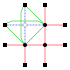
\includegraphics[width = 0.2\textwidth]{example_straight_forwards_back_substitution/example_straight_forwards_back_substitution_panel_2}} 
& \parbox{0.2\textwidth}{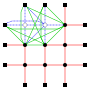
\includegraphics[width = 0.2\textwidth]{example_straight_forwards_back_substitution/example_straight_forwards_back_substitution_panel_3}} 
& \parbox{0.2\textwidth}{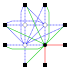
\includegraphics[width = 0.2\textwidth]{example_straight_forwards_back_substitution/example_straight_forwards_back_substitution_panel_4}} 
\end{tabular}
\end{center}

Followed by back substitution following variables in reverse order:

\begin{center}
\begin{tabular}{cccc}
\parbox{0.2\textwidth}{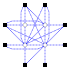
\includegraphics[width = 0.2\textwidth]{example_straight_forwards_back_substitution/example_straight_forwards_back_substitution_panel_5}} 
& \parbox{0.2\textwidth}{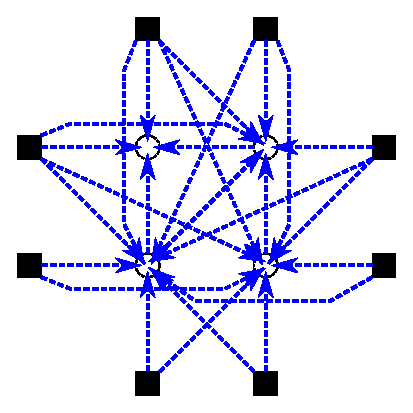
\includegraphics[width = 0.2\textwidth]{example_straight_forwards_back_substitution/example_straight_forwards_back_substitution_panel_6}} 
& \parbox{0.2\textwidth}{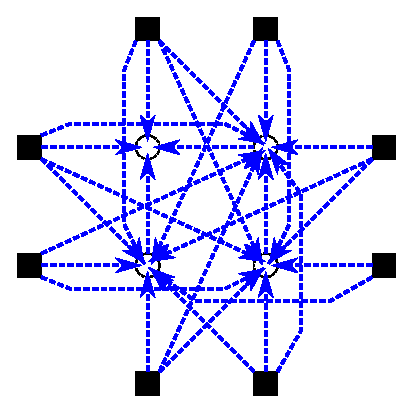
\includegraphics[width = 0.2\textwidth]{example_straight_forwards_back_substitution/example_straight_forwards_back_substitution_panel_7}} 
& \parbox{0.2\textwidth}{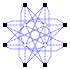
\includegraphics[width = 0.2\textwidth]{example_straight_forwards_back_substitution/example_straight_forwards_back_substitution_panel_8}} 
\end{tabular}
\end{center}





\subsection{Computational complexity}

Consider the following scenario: the computational mesh is a 3D cubic lattice where each side has dimensions of \(N\). Connections only exist between neighboring nodes. Diagonal connections do not exist. The conditioned variables are the surface of the cube, while the unknown variables are the interior of the cube. 

There are \(O(N^3)\) unknown variables in the interior of the mesh, and \(O(N^2)\) conditioned variables on the surface of the mesh. Now will be analyzed the process of performing variable elimination of each interior node, in a row-by-row, layer-by-layer process. At each step, the node to be eliminated is connected to \(O(N^2)\) other nodes via two-way connections. With the use of sparse matrices, each elimination step costs \(O(N^4)\) flops. With the elimination of \(O(N^3)\) nodes, the total computational complexity of variable elimination is: 

\[O(N^3) \times O(N^4) = O(N^7)\] 

With regards to back substitution, most nodes depend on \(O(N^2)\) other nodes. Substituting the expressions of the other nodes, each of which has a size of \(O(N^2)\), into the expression of the current node costs \(O(N^4)\) flops. In total, the computational complexity of back substitution is: 

 \[O(N^3) \times O(N^4) = O(N^7)\]

A simple mathematical model yields that when eliminating variables in a row-by-row, layer-by-layer process, the exact number of multiplication flops for {\bf variable elimination} is approximately \(4 \cdot N^7\). For this approximation to be accurate, \(N > 40\).






\section{Nested dissection}

With nested dissection, first proposed in \cite{[George1973]}, the set of variables/nodes is recursively partitioned into smaller and smaller sets. At each step a set of nodes, referred to as a ``node cluster" (terminology from \cite{[Darve2009]}), is divided into two smaller node clusters in a manner such that the sizes of the two child node clusters are approximately equal, and the number of edges connecting the two child node clusters is minimized. An example of such a partition involving an \(8 \times 8\) mesh is depicted below:

\begin{center}
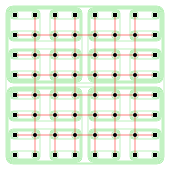
\includegraphics[width = 0.5\textwidth]{example_nested_dissection/example_nested_dissection_elimination_panel_1}
\end{center}

Node clusters that are not further partitioned are referred to as leaf node clusters. 

A node cluster is a set of nodes. Within a node cluster, there are two partitions. Provided that the node cluster is not a ``leaf" node cluster, there is the partition of the nodes between the two children of the current node cluster. In the case of all node clusters, there is a partition between the ``interior" and ``boundary" of a node cluster.  

The ``boundary" nodes of a node cluster are either conditioned nodes, or nodes that have an edge that connects to a node outside of the node cluster. The ``interior" nodes are neither conditioned nodes, nor nodes that have any connection with outside of the node cluster. In the image below, the gray box covers the interior nodes. On the left, the boundary nodes have connections to outside of the node cluster, while on the right, the boundary nodes correspond to conditioned variables, denoted by squares.

\begin{center}
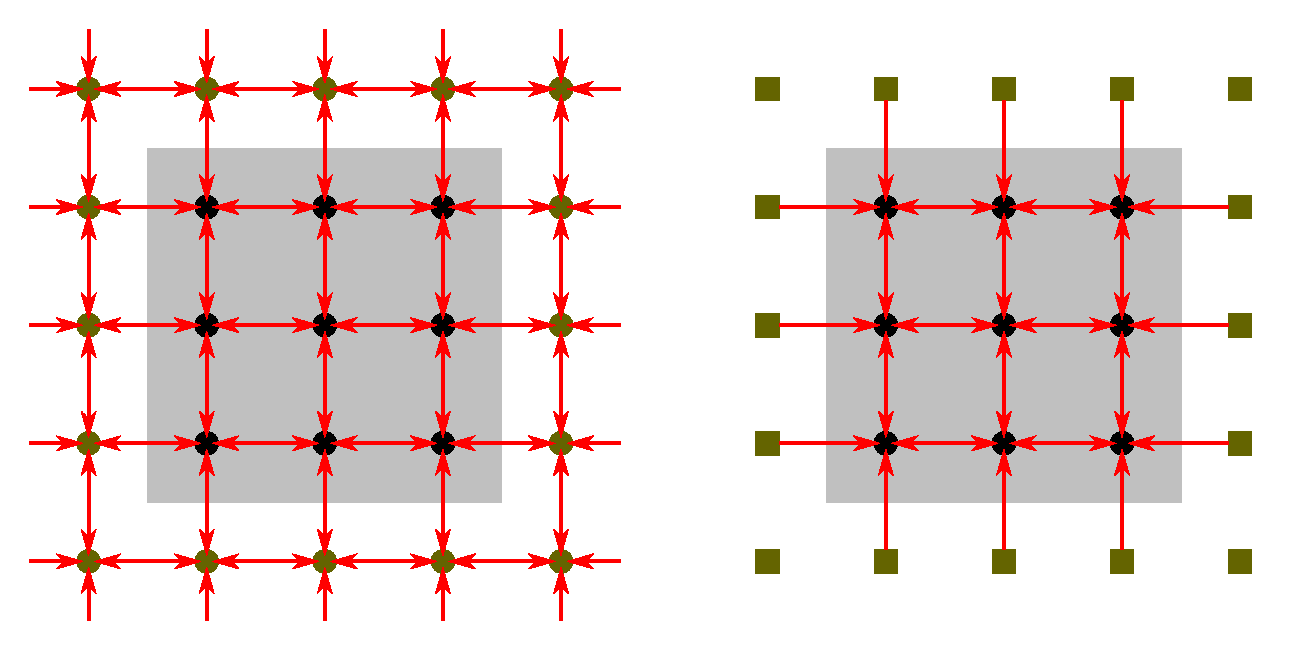
\includegraphics[width = 0.75\textwidth]{node_cluster_interior_and_boundary}
\end{center}

During the process of variable elimination using nested dissection, the interior of each node cluster is eliminated in a recursive manner. Given a node cluster, the interior of both child node clusters are eliminated prior to eliminating what remains of the current node cluster. The interior of a node cluster that is not also part of the interior of either child node cluster is referred to as the ``private interior" of the current node cluster, and it is the private interior that remains to be eliminated after the interiors of both child node clusters are eliminated. Below on the left is depicted a large node cluster that is comprised of two smaller node clusters. Below in the middle is the aftermath of eliminating the interiors of both child node clusters (the eliminated nodes are not shown). Below on the right, the private interior is highlighted, and is slated for elimination. It is important to note that with regards to leaf node clusters, the private interior is merely the interior, and this interior is simply eliminated.

\begin{center}
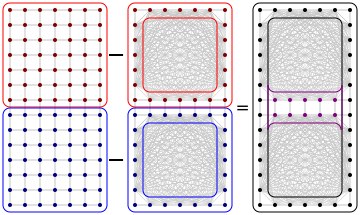
\includegraphics[width = 0.75\textwidth]{node_clusters_private_interior}
\end{center}

In the image below, one possible ordering in which the unknown variable nodes are to be eliminated using nested dissection. The conditioned variables are denoted by squares. 

\begin{center}
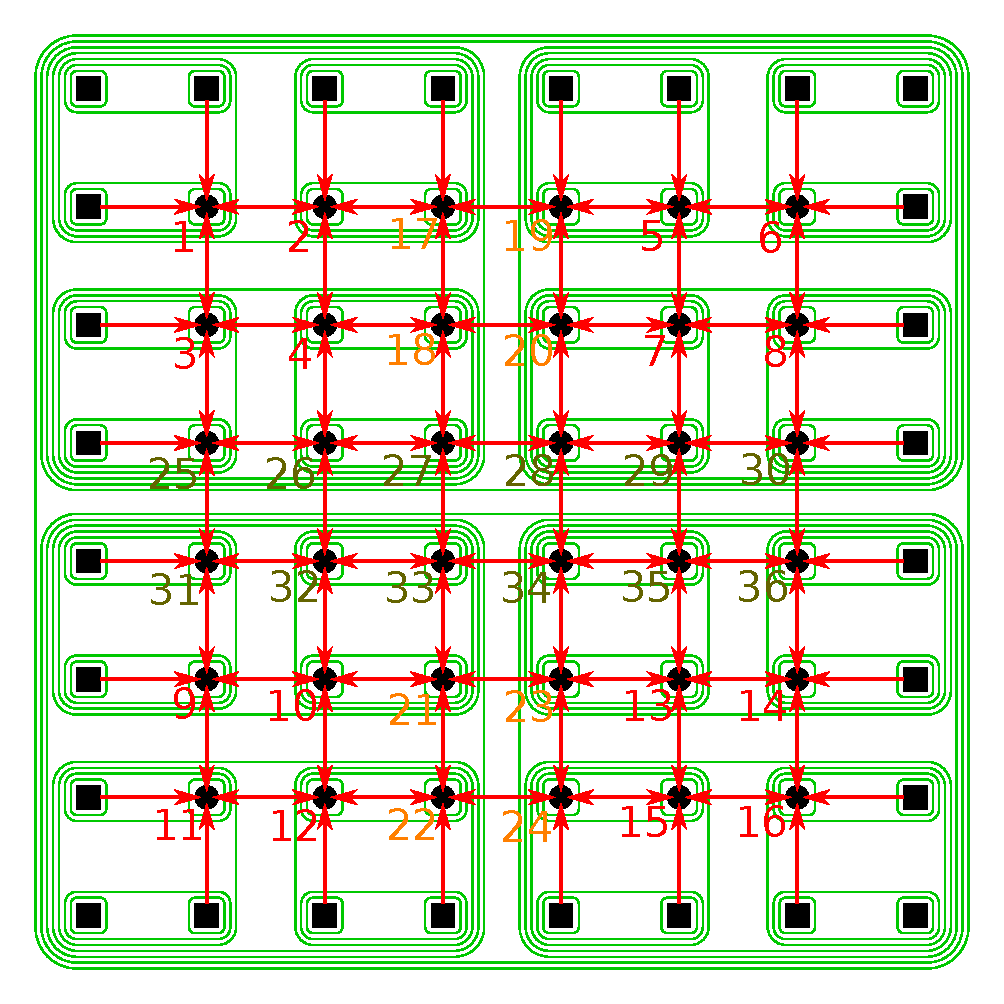
\includegraphics[width = 0.5\textwidth]{example_nested_dissection/example_nested_dissection_elimination_order_no_boundary}
\end{center}

The step-by-step process of variable elimination via nested dissection is illustrated below: 

\begin{center}
\begin{tabular}{cc} 
\parbox{0.5\textwidth}{ 
Prior to any variable elimination. There are 6 levels of partitions. In the bottom 4 levels, the node clusters do not have private interiors, so ``eliminating" the private interiors at these levels results in no change.  
} & \parbox{0.4\textwidth}{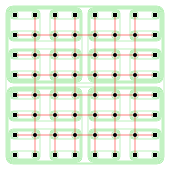
\includegraphics[width = 0.4\textwidth]{example_nested_dissection/example_nested_dissection_elimination_panel_1}} 
\end{tabular}

\begin{tabular}{cc}
\parbox{0.5\textwidth}{ 
The aftermath of eliminating the private interiors of the node clusters at level 2 of the partition. The transparent nodes are the nodes that have been eliminated. The nodes inside bubbles are all freely connected by edges (not all connections may exist though), which have been omitted for simplicity. Links between two bubbles allow for any edges in the preferred direction to exist.   
} & \parbox{0.4\textwidth}{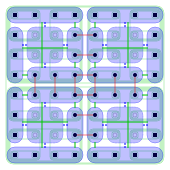
\includegraphics[width = 0.4\textwidth]{example_nested_dissection/example_nested_dissection_elimination_panel_2}} 
\end{tabular}

\begin{tabular}{cc}
\parbox{0.5\textwidth}{ 
The aftermath of eliminating the private interiors of the node clusters at level 1 of the partition.  
} & \parbox{0.4\textwidth}{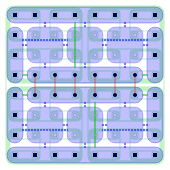
\includegraphics[width = 0.4\textwidth]{example_nested_dissection/example_nested_dissection_elimination_panel_3}} 
\end{tabular}

\begin{tabular}{cc}
\parbox{0.5\textwidth}{ 
The aftermath of eliminating the private interiors of the node clusters at level 0 of the partition. All nodes corresponding to unknown variables have been eliminated. 
} & \parbox{0.4\textwidth}{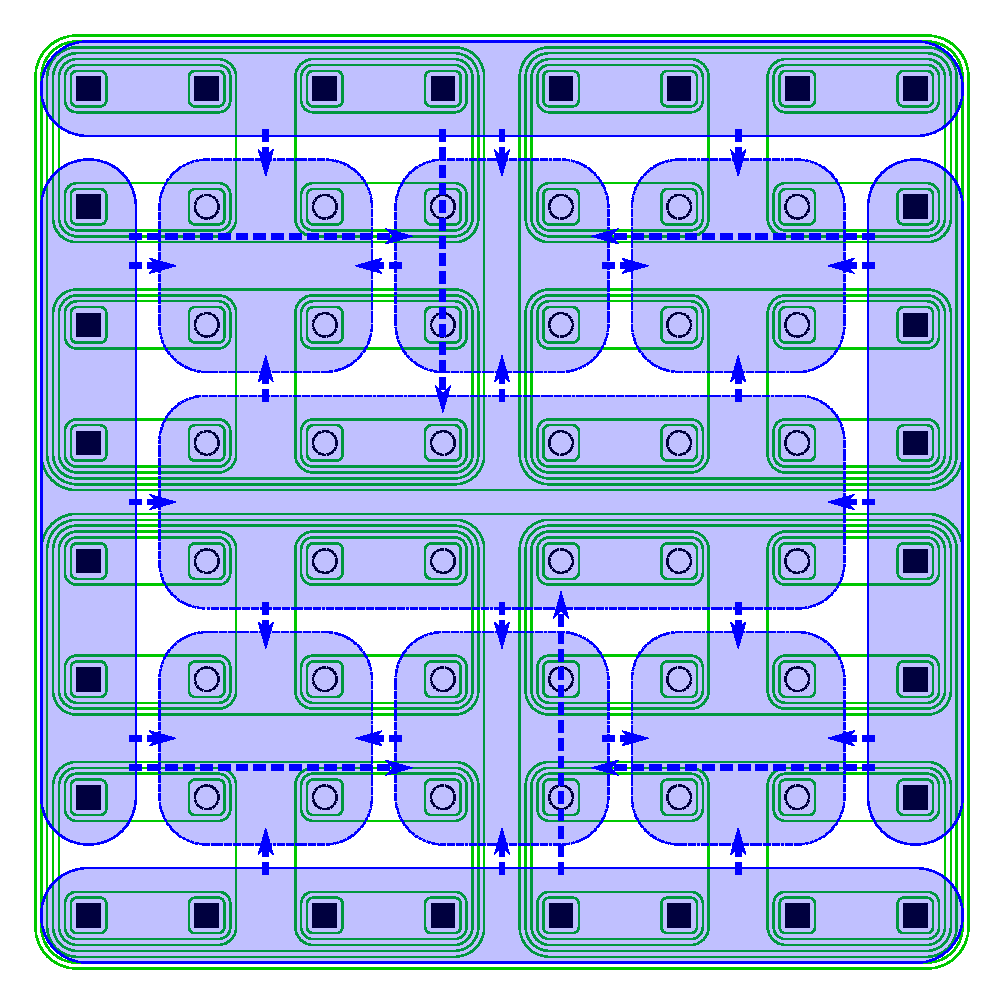
\includegraphics[width = 0.4\textwidth]{example_nested_dissection/example_nested_dissection_elimination_panel_4}} 
\end{tabular}
\end{center}



\subsection{Computational complexity}

Consider again the same scenario: the computational mesh is a 3D cubic lattice where each side has dimensions of \(N\). Connections only exist between neighboring nodes. Diagonal connections do not exist. The conditioned variables are the surface of the cube, while the unknown variables are the interior of the cube.  

This mesh will be recursively partitioned by slicing through the longest dimension, as was done in the previous examples. There will be \(O(\log(N))\) layers of partitions. At partition layer \(i\), the number of nodes in each node cluster is \(O(N^3/2^i)\), so the dimensions of each node cluster are approximately \(O(N/2^{i/3})\). Let \(M = N/2^{i/3}\). There are \(O(M^2)\) nodes in the private interior of each node cluster at partition layer \(i\), and each of these nodes is connected to \(O(M^2)\) other nodes. The flops required to eliminate each node is \(O(M^4)\), so the total flops required to eliminate the private interior of each node cluster at partition layer \(i\) is \(O(M^2) \times O(M^4) = O(M^6)\). The total flops required at partition layer \(i\), summing all possible node clusters at partition layer \(i\), is: 
\[2^i \times O(M^6) = 2^i \times O(N^6/2^{2i}) = O(N^6/2^i)\]
The total number of flops is the sum of a geometric progression where the largest term is at partition layer \(i = 0\). The total number of flops for variable elimination is therefore: 

\[O(N^6)\]

With regards to back substitution, each node in the private interior at partition layer \(i\) depends on \(O(M^2)\) other nodes where \(M = N/2^{i/3}\). Substituting the expressions of the other nodes, each of which has a size of \(O(N^2)\), into the expression of the current node costs \(O(M^2 N^2)\) flops. For the current private interior, which has a size of \(O(M^2)\), the total cost is \(O(M^4 N^2)\). The total flops required at partition layer \(i\), summing all possible node clusters at partition layer \(i\), is: 
\[2^i \times O(M^4 N^2) = 2^i \times O(N^6/2^{(4/3)i}) = O(N^6/2^{i/3})\]
The total number of flops is the sum of a geometric progression where the largest term is at partition layer \(i = 0\). The total number of flops for back substitution is therefore: 

\[O(N^6)\]

A simple mathematical model yields that the exact number of multiplication flops is approximately \(19 \cdot N^6\) for {\bf variable elimination}. The assumption being made is that the double layer of nodes that form the private interior is eliminated starting with the first layer before connecting the two interiors. For this approximation to be accurate, \(N > 40\).



\subsection{Final remarks}

The final benefit of nested dissection is that the calculations made can be used to assist in computing the solution for larger problems, especially when the same components appear multiple times. The partitioning simply has to isolate repeating components. The solution computed for each component is reused whenever the component reappears. In the image below, the same components are repeated multiple times. The red and blue lines form the boundaries of the node clusters that represent each component. 

\begin{center}
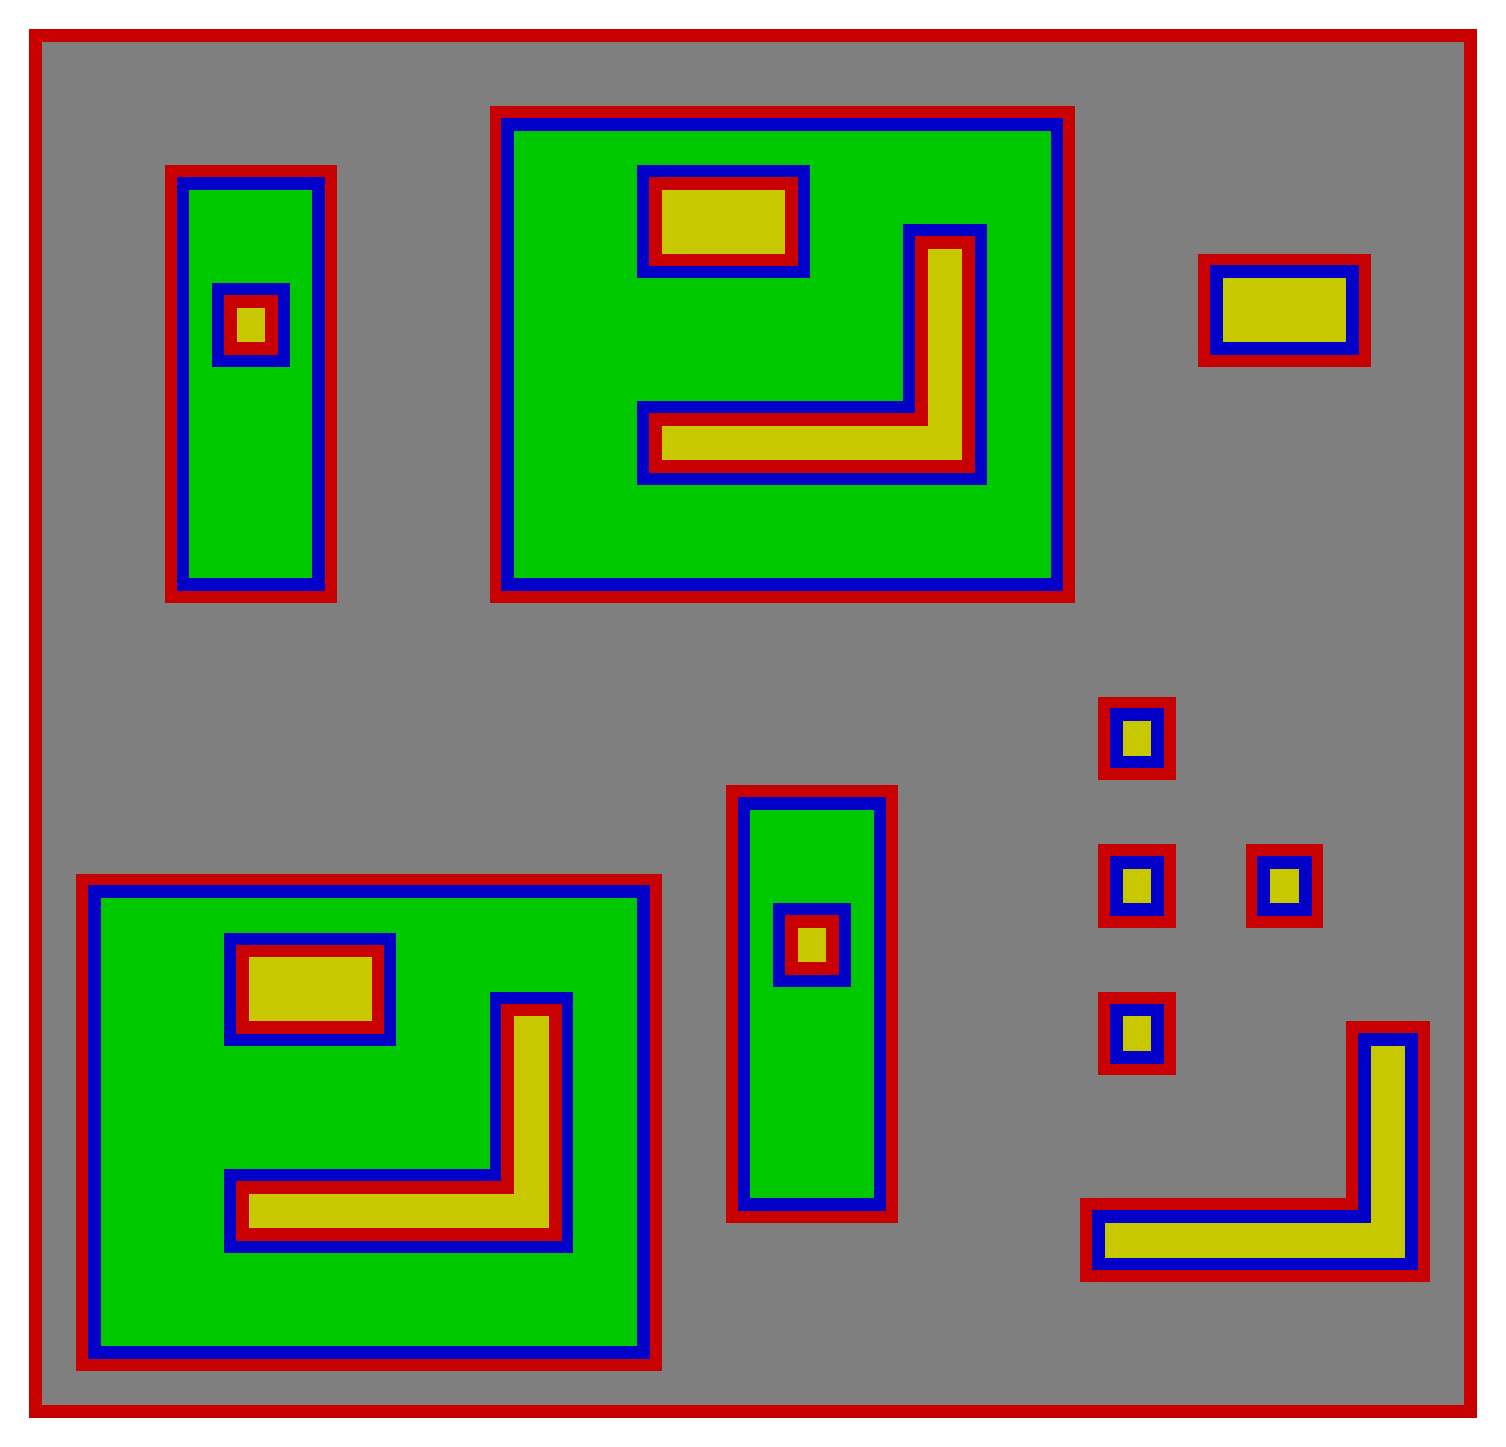
\includegraphics[width = 0.6\textwidth]{scenario_partitioning}
\end{center}






\section{Conclusion} 

In summary, the problem of computing the interior voltages of a volume given the voltages on the boundary has been analyzed via multiple approaches. If the mesh's dimensions have the scale of \(O(N)\), then computing the \(O(N^3) \times O(N^2)\) solution matrix requires: 
\begin{itemize}
\item \(O(N^9)\) flops without exploiting any sparse structure, resulting in \(O(N^4)\) flops per entry of the solution matrix.
\item \(O(N^7)\) flops directly exploiting the sparse structure, resulting in \(O(N^2)\) flops per entry of the solution matrix. 
\item \(O(N^6)\) flops using nested dissection, resulting in \(O(N)\) flops per entry of the solution matrix.
\end{itemize}

With regards to a cubic mesh with side lengths of \(N\), layer by layer variable elimination resulted in an approximate number of \(4 \cdot N^7\) multiplication flops for variable elimination alone; and nested dissection resulted in an approximate number of \(19 \cdot N^6\) multiplication flops for variable elimination alone. The assumption made in these approximations is that \(N > 40\).  

Lastly, the reusability of the calculations made with nested dissection was discussed. 



\begin{thebibliography}{9}

\bibitem{[George1973]}
George A. Nested dissection of a regular finite element mesh. \emph{SIAM Journal on Numerical Analysis} 1973; 10(2):345–363.

\bibitem{[Darve2009]}
Darve E, et al. A hybrid method for the parallel computation of Green’s functions. \emph{Journal of Computational Physics} 2009; 228:5020–5039.

\end{thebibliography}


\end{document}


























